
\section{Collider Definitions and Coordinate Systems}

\section{The Large Hadron Collider}

\section{The ATLAS Detector}

\section{Event Reconstruction}
\label{sec:event_reconstruction}

\subsection{Tracks}

\subsection{Jets}

For example, the differentiable cross-section of the ($2\rightarrow n+1$) process in \Cref{fig:quark_gluon} in the extreme soft and collinear limits factorizes into a $2 \rightarrow n$ process times a $1 \rightarrow 2$ split.
In this extreme limit the probability for soft-colinear gluon emission is given by,
\begin{equation}
	\label{eq:gluon_emission}
	d \mathcal{S} = \frac{2 \alpha_s C_F}{\pi} \frac{d \theta}{\sin\theta} \frac{dE}{E} \frac{d\phi}{2\pi},
\end{equation}
where $C_F = \sfrac{4}{3}$ is the color factor for the quarks, $\theta$ is the angle of the emitted gluon with respect to the quark, $E$ is the energy of the emitted gluon, and $\phi$ is the azimuthal angle.

\subsubsection{Particle Flow}
\label{sec:particle_flow}

\subsubsection{Fat Jets}
At the LHC, quarks can be produced in the decays of particles such as $W/Z$~bosons, or top quarks through their decay into a $W$~boson and a $b$-quark.
For most energy scales, the two or three quarks from these decays produce jets that can be individually resolved in the detector.
However, as the momenta of the intermediate particles increase, the decay products themselves start to collimate, resulting in a single large-radius or \textit{fat} jet in the detector; this is the so-called boosted regime.
These objects are colloquially referred to as \textit{fat jets}.
The vast majority of jets, however, are initiated by partons, which are not the decay products of other massive particles (QCD background).

\subsection{Jet substructure}
\label{sec:jet_substructure}

Properties relating to the distribution of constituents within a jet are known as the substructure of a jet, which can be used to identify the original seed particle~\cite{Kogler:2018hem}.
This is particularly interesting in the boosted regime, where several partons from the decay of another elementary particle have overlapping showers.
% In boosted topologies it is of particular interest to identify whether a jet is from hadronic decays of a resonant particle or otherwise.
% Therefore, accurate modelling of jet substructure is of importance in many measurements and searches at the LHC.
% Many high level features are defined based on physics principles and are calculated from the constituents in a jet.

One commonly used set of observables to describe jet substructure is its \emph{N-subjettiness}~\cite{Thaler_2011}, denoted by ${\tau_N}$.
These are useful in identifying jets originating from processes with $N$ prongs as a result of the decay of the initial particle.
A jet originating from a gluon is likely to have a 1-prong substructure, whereas a $W/Z$~boson decay is likely to produce a 2-prong jet, and a jet originating from the all-hadronic decay of a top quark will tend to be 3-prong.
Other commonly used observables relate to the energy correlation functions of a jet and their ratios, such as $D_2$~\cite{Larkoski_2013,Larkoski_2014}.%
\footnote{$D_2$ is defined as the ratio of the three-point and cubed two-point energy correlation functions.}
A new set of features which have been found to be sensitive to the underlying substructure of different jet types are the Energy Flow Polynomials~(EFPs)~\cite{Komiske_2018}.

Furthermore, when a seed particle decays, the observed opening angle of the decay products is strongly dependent on its mass and momentum.
In jets, this means that the distribution of constituent properties is strongly correlated to the overall invariant mass and transverse momentum \pt.

Classification approaches applying cuts on the substructure features, as well as machine learning algorithms trained using such features have been successfully employed in the ATLAS and CMS collaborations to distinguish jets originating from $W$~bosons ($W$-jets), top quarks (top jets), gluons, and light quarks~\cite{ATLAS:2018wis,CMS:2020poo}.
In recent years, more sophisticated classification algorithms have been trained on the constituents themselves, either represented as ordered vectors~\cite{pearkes2017jet,ATLAS:2018wis,CMS:2020poo,Butter_2018}, images~\cite{de_Oliveira_2016,Kasieczka_2017,Macaluso_2018}, or point clouds~\cite{ParticleNet,Komiske:2018cqr,Moreno:2019bmu,Dreyer:2020brq,Dolan:2020qkr,Mikuni:2021pou,Shimmin:2021pkm,Gong:2022lye,Qu:2022mxj} (see Ref.~\cite{TopLandscape} for a review).

These approaches are very sensitive to the substructure of jets originating from different particles.
As such, when using fast surrogate models it is crucial that they accurately capture the distribution of the constituents within a jet and their correlations to the mass and \pt.

% This is also apparent for jets originating from a top quark, which are often reconstructed without full containment of all three decay products in a single jet.
% This results in only the decays of a $W$~boson being captured within a jet, and as such the substructure changes drastically for lower jet masses.


\section{Event Simulation}

\section{Flavour Tagging}

A diagram of the GN1 model is shown in \Cref{fig:gn1}.

\begin{figure}
    \centering
    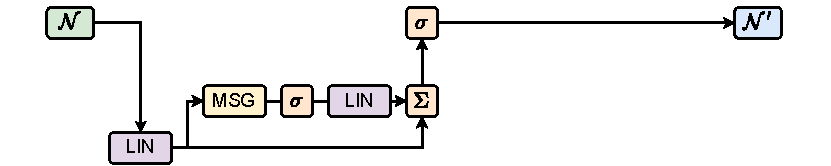
\includegraphics[width=0.99\textwidth]{figures/atlas/gn1.png}
    \caption{Schematic diagram of the GN1 model from Ref.~\cite{GN1}.}
    \label{fig:gn1}
\end{figure}
